\documentclass[11pt,a4paper]{article}
\usepackage[margin=2cm]{geometry}
\usepackage{booktabs,tabularx,array,enumitem,xcolor,hyperref,listings,amsmath,graphicx}
\usepackage[T1]{fontenc}
\usepackage{lmodern}
\hypersetup{colorlinks=true,linkcolor=blue!50!black,urlcolor=blue!50!black}
\newcolumntype{L}{>{\raggedright\arraybackslash}X}
\setlist{nosep,leftmargin=*}
\setlength{\emergencystretch}{3em}
\lstset{language=C,basicstyle=\ttfamily\footnotesize,breaklines=true,columns=fullflexible,keepspaces=true,
  frame=single,framerule=0.3pt,rulecolor=\color{black!30},xleftmargin=2pt,xrightmargin=2pt,
  commentstyle=\color{green!40!black},keywordstyle=\color{blue!60!black},showstringspaces=false}
\newcommand{\lv}[1]{\texttt{#1}}                 % a Live Expressions variable
\newcommand{\run}[1]{\textbf{How to run.} #1}
\newcommand{\see}[1]{\textbf{What you see.} #1}
\newcommand{\tbm}{\textcolor{red}{[to measure]}}  % a number not yet measured on the board
\newcommand{\flag}[1]{\textcolor{red}{[#1]}}

\title{Microprocessor-Based Product Design 2026/27\\[2pt]\large Assignment 2: reference solution}
\author{Yohai Ackerman (TA). \textbf{TA only, never handed to students.}}
\date{Draft of \today}

\begin{document}
\maketitle

\section{The project and how to operate it}

\subsection{What is where}
Everything is in \texttt{assignments/ass2/solution/fullSolution/}:

\smallskip\noindent
\begin{tabularx}{\textwidth}{@{}l L@{}}
\toprule
File & Content \\
\midrule
\texttt{ass2\_sol.tex} & this document \\
\texttt{ass2\_sol/} & the STM32CubeIDE project \\
\texttt{ass2\_sol/ass2\_sol.ioc} & the TA's \texttt{ass2.ioc}: \texttt{ass1.ioc} plus everything in ``Assignment 2: project
  configuration'' (never given to students) \\
\texttt{Core/Src/main.c} & generated code; the user code adds \texttt{\_\_io\_putchar}, declares \lv{task}
  (\texttt{volatile uint16\_t}, \texttt{USER CODE BEGIN PV}), calls \texttt{ass2Init()} in \texttt{USER CODE BEGIN 2}
  and the dispatcher in the main loop \\
\texttt{io\_board.c/.h}, \texttt{sonar.c/.h} & the students' copies, unchanged \\
\texttt{Core/Inc/ass2.h} & task numbers, wheel helpers, shared helpers \\
\texttt{Core/Src/ass2\_tasks.c} & start-up, the dispatcher, \texttt{allOff()}, and the three HAL callbacks \\
\texttt{Core/Src/ass2\_common.c} & \texttt{taskDone}, \texttt{waitMs}, \texttt{printFixed2}, the pass counter, wheel~1,
  \texttt{encoderSetMode} \\
\texttt{Core/Src/partA.c} \ldots\ \texttt{partE.c} & one file per part \\
\bottomrule
\end{tabularx}

\smallskip\noindent
\texttt{ass2\_sol.ioc} was written from \texttt{ass1.ioc} and generated with CubeMX 6.18.1 headless. CubeMX 6.18.1
asks to migrate a 6.18.0 file (in the GUI it is a question; headless it hangs), so the file says 6.18.1. Checked in the
generated code: TIM2 PSC 0 / ARR 9\,999, TIM1/3/4/8 encoder TI1 with ARR 65\,535, TIM5 PSC 9 / ARR 1\,699\,999 with
CH2 on both edges, TIM6 169 / 9\,999, TIM7 169 / 99, PA7 EXTI on both edges, DIR1 to DIR4 outputs, low. One
difference from the configuration section: the generated TIM5 CH1 pulse is 0, not 170. It does not matter, because
\texttt{sonar.c} writes 170 before it starts the trigger.

\subsection{Opening, building and starting a debug session}
As in Assignment~1: import \texttt{fullSolution/ass2\_sol} into STM32CubeIDE, build (Debug), cart power on with the
jumper on E5V, \textbf{the cart on its block}, PuTTY at 115\,200 8N1, start the debug session with
\texttt{ass2\_sol Debug.launch}, Resume, and add \lv{task} (and \lv{pwmN}, \lv{pwmM} for Part~A) to Live
Expressions. PuTTY shows the IO board report and the menu.

\subsection{Choosing a task}
The protocol of Assignment~1, with three-digit numbers: write the number into \lv{task}; \texttt{=== task N ===}; a
task with an end prints \texttt{=== task N done ===}; write 0 and the number again to repeat it. After every task,
\texttt{allOff()} stops all four wheels (CCR1 to CCR4 = 0), stops TIM6 and TIM7 (and returns TIM7 to 10\,kHz), stops
the ultrasonic sensor (\texttt{sonarStop()}), disables the IR interrupt, sets the four encoders back to TI1 (the
\texttt{.ioc} setting; D.2 and E set TI1 and TI2 themselves), and switches LD2 and the RGB LEDs off.

\smallskip\noindent
\begin{tabularx}{\textwidth}{@{}c L c L@{}}
\toprule
\lv{task} & Runs & \lv{task} & Runs \\
\midrule
111 & A.1.1 polling PWM on LD2 & 310 & C.1 bus scan \\
112 & A.1.2 the same, $M = N/2$ & 320 & C.2 own PCA9634 driver, 8 colours \\
121 & A.2.1 TIM7 PWM on LD2 & 330 & C.3 8 writes vs.\ one burst \\
122 & A.2.2 TIM7 PWM on wheel~1 & 340 & C.4 buttons and HAL return values \\
123 & A.2.3 TIM7 at 10\,kHz, then 1.7\,MHz & 350 & C.5 servo \\
124 & A.2.4 1000 \texttt{setLedChannel} calls & 411 & D.1.1 by hand, TI1 \\
131 & A.3.1 TIM2 duty sweep & 412 & D.1.2 by hand, TI1 and TI2 \\
132 & A.3.2 PCA9634 PWM, wheel at 50\,\% & 413 & D.1.3 motor, 8\,s in each mode \\
210 & B.1 ultrasonic raw readings & 420 & D.2 speed, two ways (TI1 and TI2) \\
221 & B.2.1 IR hand passes, polling & 510 & E.1 the four wheels (B1 runs the next) \\
222 & B.2.2 IR hand passes, interrupts & 521 to 524 & E.2.1 to E.2.4 step of wheels 1 to 4 \\
231 & B.3.1 ultrasonic hand passes, polling & & \\
232 & B.3.2 ultrasonic hand passes, interrupts & & \\
\bottomrule
\end{tabularx}

\subsection{Status of this solution}
\textcolor{red}{\textbf{2026-11-05: the instructions were shortened and Parts B, D.1 and E restructured} (B.2 = the IR
test and B.3 = the ultrasonic test, each by polling and by interrupts, ended by B1; D.1.1/D.1.2 by hand in each mode
and D.1.3 one 8\,s motor run per mode; D.2 and E in TI1 and TI2; E for all four wheels). The code follows the new text and builds with 0 warnings. \textbf{All the new tasks were run on the cart on
2026-11-05} with Yohai: B.2 on the first cart, then (after the change to one sensor per task) B.3, D.1.2, D.1.3,
D.2, E.1 and E.2 on a second cart, where motor~4's forward level is RESET. The automatic test of the new version
(2026-11-05) passed every item here and caught the four planted errors of the wrong copy.}

\smallskip\noindent
The code builds with the CubeIDE toolchain (GCC 14.3, Debug) with 0 warnings (2026-11-05). \textbf{Run on the cart
twice.} On 2026-10-29, wheels in the air, every task was started over SWD with no hand on the cart; the log is in
\texttt{assignments/autotest/logs/ass2/} (git-ignored). On 2026-11-04 the tasks that need a hand, an obstacle or
eyes were run with Yohai at the cart: the B.1 distances, the hand passes of test~1, the C.4 buttons, the servo of C.5,
the D.1 hand turns; D.1.2 (now with the motor), D.2 (now one direction until two wraps), B.2/B.3 tests 2 and 3 and
E.1 were run again. ``Measured'' numbers are from 2026-11-04 unless the date says otherwise. The constants found on
the cart:
\begin{itemize}
  \item \texttt{COUNTS\_PER\_REV\_TI1} (\texttt{ass2.h}) = 660 (D.1.1), and \texttt{COUNTS\_PER\_REV} = 1\,320 in TI1
        and TI2, the mode used from D.2 on (the factor 2.00 to 2.01 of 2026-11-04; D.1.2 by hand: 1\,320.2, 2026-11-05).
  \item The wheel table \texttt{wheels[4]} (\texttt{ass2\_common.c}): motor channel, DIR pin and forward level, encoder
        timer, and the sign that makes forward positive. Measured in E.1 (2026-11-05, the second cart): forward is
        SET for motor~1 and RESET for motors 2, 3 \textbf{and 4} (the configuration section says SET for motor~4:
        not so on this cart), and the signs are $-1, +1, -1, +1$.
  \item \texttt{RAW\_PER\_MM\_X10} (\texttt{partB.c}) = 1019 (B.1; the theory gives 991).
  \item \texttt{SERVO\_CHANNEL} (\texttt{partC.c}) = 0 (C.5: seen moving on channel~0 only).
  \item \texttt{IR\_OBSTACLE\_LEVEL} (\texttt{ass2.h}) = \texttt{GPIO\_PIN\_SET}: on this cart the IR sensor gives HIGH
        for an obstacle (A1 Part~E).
\end{itemize}
The flicker and the sound of Part~A and the colours of C.2 were checked by Yohai on 2026-11-05 (the second cart, wheels in the air).
\textbf{On this cart, wheel~1 forward makes TIM1 count down}; from 2026-11-05 the code multiplies by the sign of the
wheel table, so forward speeds are positive (the 2026-11-04 numbers below are still negative).

\section{Shared pieces}
\begin{lstlisting}
void wheel1Duty(uint32_t percent) { TIM2->CCR1 = percent * PWM_FULL / 100u; }   // PWM_FULL = 10000
void wheel1Forward(uint8_t forward)            // DIR1: SET is forward for motors 1 and 4
{ HAL_GPIO_WritePin(DIR1_GPIO_Port, DIR1_Pin, forward ? GPIO_PIN_SET : GPIO_PIN_RESET); }

void encoderSetMode(uint32_t mode)             // D.1, at run time
{
    HAL_TIM_Encoder_Stop(&htim1, TIM_CHANNEL_ALL);
    TIM1->SMCR = (TIM1->SMCR & ~TIM_SMCR_SMS) | mode;
    TIM1->CNT  = 0;
    HAL_TIM_Encoder_Start(&htim1, TIM_CHANNEL_ALL);
}
\end{lstlisting}
\texttt{printFixed2(v)} prints two decimals as two integers, so newlib-nano needs no float support. The callbacks
(\texttt{ass2\_tasks.c}) pass each event on: TIM7 to A.2, TIM6 to D.2 or E, the TIM5 capture to B (through
\texttt{sonarCaptureEdge}), and the EXTI of PA7 to the interrupt tasks of B. B1's EXTI (PC13) is ignored; B1 is read
by polling (\texttt{b1Pressed()}, HIGH while pressed, one event per press) where a task needs it.

\section{Part A: three ways to make a PWM}
Symbols: $N$ steps per period, $M$ of them on, $f_\mathrm{PWM} = 1/(N\,t_\mathrm{step})$, duty $= M/N$, $N + 1$ duty
levels (0 to $N$). Every task of A.1 and A.2.1 to A.2.3 prints \texttt{Ax.y: N=100 M=50 passes=<n>} once a second.

\subsection*{A.1 Polling (\lv{task} 111, 112)}
\begin{lstlisting}
uint32_t step = HAL_GetTick() % n;                       // 0 .. N-1, one step per ms
HAL_GPIO_WritePin(LD2_GPIO_Port, LD2_Pin, (step < pwmM) ? GPIO_PIN_SET : GPIO_PIN_RESET);
\end{lstlisting}
\textbf{A.1.1.} $t_\mathrm{step} = 1$\,ms, $N = 100$: $f_\mathrm{PWM} = 10$\,Hz. The LED visibly blinks at 10\,Hz,
and the duty changes the on time: $M = 0$ is off, $M = 100$ is on, in between it blinks with a longer or shorter
flash. Passes per second, measured: 904\,000 (1.1\,$\mu$s per pass of \texttt{HAL\_GetTick}, \texttt{\%} and
\texttt{HAL\_GPIO\_WritePin}), the same at $N = 100$ and $N = 20$.

\emph{What the passes mean} (the answer the instructions ask for): a pass of about 1\,$\mu$s is far shorter than
the 1\,ms step, so the loop reads every tick value about 1000 times and each edge is at most 1\,$\mu$s late. The
polling itself is fast enough. The blinking has another cause: a 1\,ms step with $N = 100$ gives $f_\mathrm{PWM} =
1/(100 \times 1\,\mathrm{ms}) = 10$\,Hz, which is far too slow for the eye. If the loop also did slow work (a
\texttt{printf}, I2C), each pass could last longer than the step, and the PWM itself would break (tutorial~4,
slide 27).

\textbf{A.1.2.} The code writes $M = N/2$ (871\,000 passes per second, measured, with the extra division). Seen on the cart (Yohai, 2026-11-05): LD2 blinks at $N = 100$ and $50$
(10 and 20\,Hz), is almost steady at $N = 30$ (33\,Hz) and steady at $N = 20$ (50\,Hz), which leaves only 21 duty
levels. It depends on the eye: accept any $N$ from about 30 to 10, with the frequency it gives. The trade-off: with a fixed $t_\mathrm{step}$, a higher
$f_\mathrm{PWM}$ needs a smaller $N$, so fewer brightness levels.

\textbf{A.1.3.} $N = 1/(f_\mathrm{PWM}\,t_\mathrm{step}) = 1/(17\,000 \times 0.001) = 0.06$. A period of 59\,$\mu$s is
shorter than one 1\,ms step, so it is impossible: with \texttt{HAL\_GetTick} the fastest PWM is $N = 2$, 500\,Hz,
with one level between off and on.

\subsection*{A.2 Interrupt (\lv{task} 121 to 124)}
\begin{lstlisting}
void partA2Tick(void)                            // TIM7 update, every 100 us
{
    if (task != a2Task) { /* back to 10 kHz, stop TIM7, wheel off */ return; }
    if (++a2Step >= pwmN) a2Step = 0;
    uint8_t on = (a2Step < pwmM);
    if (a2Task == TASK_A2_1) LD2_GPIO_Port->BSRR = on ? LD2_Pin : ((uint32_t)LD2_Pin << 16);
    else                     TIM2->CCR1 = on ? PWM_FULL : 0;     // wheel 1 fully on or off
}
\end{lstlisting}
\textbf{A.2.1.} $f_\mathrm{PWM} = 1/(100 \times 100\,\mu\mathrm{s}) = 100$\,Hz: no visible flicker, with all 101
levels. Measured: 1\,850\,000 passes per second (this loop does less than A.1's, so it is faster). The same loop
without TIM7 (A.3.2) makes 2\,120\,000, so the 10\,kHz interrupt takes about 13\,\% of the CPU: about 13\,$\mu$s per
interrupt in this Debug build (HAL handler and callback at \texttt{-O0}). That is far more than the 1\,$\mu$s in
tutorial~4's examples, which is only an example value. The real time depends on the code and the build, and the
passes per second are how the students find it. Expect answers of the same order as 13\,$\mu$s.

\textbf{A.2.2.} $N = 100$: 100\,Hz on the wheel, 5\,ms full on and 5\,ms off. $N = 10$: 1\,kHz. Both are well
inside the audible range. \textbf{Heard on the cart} (Yohai, 2026-11-05, wheels in the air): at both the wheel
turns smoothly and the sound is acceptable; at 1\,kHz it sounds a little different. The gearbox makes most of the
noise, so the PWM's own tone is hard to pick out. So do not expect a jerky wheel or a loud hum: grade an honest
description together with the reasoning (100\,Hz and 1\,kHz can be heard, the motor's mass smooths the speed).

\textbf{A.2.3.} 17\,kHz with $N = 100$ needs 1.7\,MHz steps: $170\,\mathrm{MHz}/1.7\,\mathrm{MHz} = 100$ timer clocks,
so PSC = 0 and ARR = 99. It does not work: 100 CPU cycles per interrupt is less than the HAL interrupt handler and the
callback take, so the CPU is always in the interrupt. Updates are lost, and the PWM comes out slower and irregular.
The main loop never runs. Measured: at 10\,kHz the loop made 1\,385\,000 passes per second, but after the switch
PuTTY printed nothing at all, not even \texttt{A2.3: TIM7 PSC=0 ARR=99}, for the 3\,s until \lv{task} was changed.
Then the callback stopped TIM7 by itself, and the waiting lines came out. SysTick still runs: it has the same priority
(0) and a lower exception number, so it wins ties. Seen on the cart (2026-11-05): after the switch the main loop made
\textbf{1 pass in 23\,s}, yet the wheel kept turning and looked normal, only sounding a little different. The
steps come slower and unevenly, but still about half of them on, and the wheel smooths that out. So the failure
shows in the passes and the silent PuTTY, not in the wheel: do not expect students to see the wheel misbehave.

\textbf{A.2.4.} Measured: \texttt{A2.4: calls=1000 ms=75}. One write is start, address, register
and data (3 bytes with their ACKs: 27 bits) and stop, about 29 bit times of 2.5\,$\mu$s = 73\,$\mu$s, plus the HAL code.
One LED update takes about 80\,$\mu$s, almost the whole 100\,$\mu$s step, and all 24 channels take about 2\,ms. A
callback must take far less than the step. Besides, the HAL I2C functions block and wait on \texttt{HAL\_GetTick},
and an I2C transfer started inside an interrupt would collide with one that the main loop has under way.

\subsection*{A.3 Hardware (\lv{task} 131, 132)}
\textbf{A.3.1.} TIM2 runs at $170\,\mathrm{MHz}/10\,000 = 17$\,kHz with 10\,001 levels, and the CPU writes CCR1 once
per step: \texttt{A3.1: duty=35 CCR1=3500}, 2\,s per step, 0 to 100\,\%, then the wheel stops and the task is done.
Measured from the encoder during the sweep: the wheel stands still up to 10\,\% (one count in 2\,s), and starts
turning at \textbf{15\,\%}. That is the dead zone: below it, the torque does not overcome the static friction of the
motor and gearbox. The speed then grows with the duty: about 420 counts/s at 15\,\%, 1\,050 at 30\,\%, 1\,850 at
50\,\%, 2\,700 at 70\,\% and 3\,750 at 100\,\%. 17\,kHz is at the top of the audible range. Heard on the cart (A.3.2, 50\,\%, 2026-11-05):
``pretty good, perhaps less noisy'' than the 100\,Hz and 1\,kHz of A.2.2; the gearbox still makes its noise.

\textbf{A.3.2.} LED~0 is set once (green, 64), and the PCA9634 keeps its own PWM (about 97\,kHz, from its internal
oscillator) with no further I2C traffic. Measured: 2\,120\,000 passes per second, the fastest loop of Part~A:
hardware PWM costs the CPU nothing.

\subsection*{A.4 The comparison}
\begin{tabularx}{\textwidth}{@{}l l l l L@{}}
\toprule
Method & $t_\mathrm{step}$ & $f_\mathrm{PWM}$ & $N$ & CPU cost and result \\
\midrule
1 polling & 1\,ms & 10\,Hz ($N = 100$) & 100 & the loop does nothing else (904\,000 passes/s); LED flickers; no motor PWM \\
2 interrupt & 100\,$\mu$s & 100\,Hz & 100 & about 13\,\% at 10\,kHz (1\,850\,000 passes/s), 100\,\% at 1.7\,MHz (0 passes); LED fine, motor loud \\
3 hardware & 5.9\,ns & 17\,kHz & 10\,000 & none (2\,120\,000 passes/s); motor quiet, fine resolution \\
PCA9634 & (chip) & about 97\,kHz & 256 & none after one I2C write; the RGB LEDs \\
\bottomrule
\end{tabularx}

\noindent An LED needs only above about 100\,Hz (eye), so method~2 is enough. A motor needs above 20\,kHz or close
to it (ear, and smooth current through the winding inductance), with fine resolution: only the hardware timer does it.

\section{Part B: polling vs.\ interrupts}

\subsection*{B.1 Calibration (\lv{task} 210)}
\run{Motors off. Prints \texttt{B1: raw=<n>} for every reading (10 per second) and \texttt{B1: avg=<n>} after every
10. Since 2026-11-05 the instructions prescribe no lines for B.1 (``assume a linear mapping, find its ratio, explain,
compare with theory''), so B.1 is graded from the report only; these lines are our own.}

\textbf{Answer.} TIM5 counts at $170\,\mathrm{MHz}/(9+1) = 17$\,MHz, so one count is 58.8\,ns. The echo lasts the
round trip $2d/c$:
\[
  \text{raw} = \frac{2d}{343\,000\,\mathrm{mm/s}} \cdot 17 \times 10^{6}\,\mathrm{s^{-1}} = 99.1\,d\,[\mathrm{mm}],
  \qquad d = \text{raw}/99.1 = 0.0101\,\text{mm} \times \text{raw}.
\]
\see{Measured: a book held square to the sensor at 5, 10 and 15\,cm from the front of the transducers, averages
4\,226, 10\,065 and 14\,418. The straight line through them: 101.9 counts per mm, offset $-6$\,mm. So
\texttt{RAW\_PER\_MM\_X10} = 1019, and $d \approx \text{raw}/101.9$. The slope means a speed of sound of
$2 \times 17 \times 10^{6} / 101.9 = 334$\,m/s, 3\,\% below 343\,m/s: well within the accuracy of distances held by
hand ($\pm 5$\,mm on three points). With 1019, the stop threshold of 150\,mm is a raw value of 15\,285.}

\see{Shortest distance (measured): from 5 to 25\,mm the reading stays near 2\,630 (``26\,mm'') or jumps around; from
30\,mm on it follows the distance (30\,mm: 2\,952, theory 2\,973). So the sensor measures reliably from about 30\,mm:
closer, the echo returns while it is still sending. With no obstacle placed (the cart on its block, facing the room,
2026-10-29): readings 10 per second, raw 56\,000 to 82\,000 (about 0.57 to 0.83\,m). The longest distance was not
measured (a few metres by the datasheet). With no echo, the HC-SR04 holds ECHO for about 38\,ms (raw about
646\,000), which fits within the 100\,ms trigger period (1\,700\,000 counts). The counter restart between the two
edges is handled in \texttt{sonar.c}.}

\subsection*{B.2 and B.3: the control (\lv{task} 221, 222, 231, 232)}
\begin{lstlisting}
// all four tasks, every pass
if (irObstacle || sonarNear)                        lastSeen = now;
else if (!wheelOn && now - lastSeen >= CLEAR_MS)    { wheelOn = 1; wheel1Duty(40); }
if (status changed) { setRGB(...) if wheelOn changed; printf("status wheel=%u ir=%u\r\n" or "near=%u", ...); }
HAL_Delay(150);                                     // the other work
// the loop period, averaged over each second; at every stop: "B2.1: stops=<n> period=<ms>"
if (b1Pressed()) break;                             // B1 ends the task (B3.x: then the readings line)

// one sensor per task: B.2 the IR sensor only, B.3 the ultrasonic one only (the other flag stays 0)
// x.1 (221, 231): polled once per pass  // x.2 (222, 232): in the callback
if (B.2) irObstacle = (ReadPin(IR) == IR_OBSTACLE_LEVEL);  // 222: HAL_GPIO_EXTI_Callback (both edges):
else if (sonarPoll()) sonarNear = ...;   //   irObstacle = ...; if (irObstacle) stopWheel(); lastSeen = now;
if (irObstacle || sonarNear)             // 232: HAL_TIM_IC_CaptureCallback: sonarNear = raw < NEAR_RAW;
    stopWheel();                         //   if (sonarNear) { stopWheel(); lastSeen = now; }

static void stopWheel(void) { TIM2->CCR1 = 0; if (wheelOn) { wheelOn = 0; stopCount++; } }
\end{lstlisting}
\textbf{One sensor per task} (instructions changed 2026-11-05): B.2 uses only the IR sensor and B.3 only the
ultrasonic one, so a hand near the other sensor cannot stop the wheel. 221 reads the IR pin; 222 clears any old
EXTI flag and enables \texttt{EXTI9\_5\_IRQn}; 231 starts \texttt{sonarStartPolling()}; 232 starts
\texttt{sonarStartInterrupt()}. The status line shows only that sensor (\texttt{status wheel=1 ir=0} or
\texttt{status wheel=1 near=0}). B.2 moves a hand past the IR sensor and B.3 in front of the
ultrasonic one (from about 200 to about 100\,mm and back), 10 times, about 3\,s apart, and B1 ends the task. At the
end, B.3 prints \texttt{B3.1: readings=<n> missed=<m> ms=<t>}. The callback records \texttt{lastSeen} on both IR
edges, so a hand that passes between two loop passes still holds the wheel for 1\,s.

\textbf{Loop period}: now $150\,\mathrm{ms}$ plus very little, because the LEDs and the status line are written only
when the status changes (before 2026-11-05 they were written on every pass: 155 to 156\,ms measured). Measured on 2026-11-05: 151 to
152\,ms in all four tasks, with polling and with interrupts.

\textbf{B.2, measured} (2026-11-05, the new version but still watching both sensors, old cart, loop period 151 to 152\,ms in every task): polling, hand waves
1 to 2\,s apart: 10 stops of 10; polling, quick flicks: 9 of 10; interrupts, quick flicks: 10 of 10, and for 5 of
them the main loop never saw \texttt{ir=1} (the flick was over within one loop pass), so polling could have missed
each of them. A hand that stays in front for 150\,ms or more is always seen by polling: the passes must be
\textbf{very quick} flicks (the instructions now say so), and even then the IR module may stretch a short pulse, so
the difference shows only in some of the passes. B1 ended every task.

\textbf{B.3.1, measured} (2026-11-05, one sensor per task, a second cart, 10 hand passes from about 200 to
100\,mm): \texttt{B3.1: readings=0 missed=139 ms=21146}, no stop at all. 139 passes in 21.1\,s is 152\,ms per
pass, and every pass found both edges of an echo already captured (overcapture), so polling never completed a
reading. Task 210 on the same cart showed the sensor itself working (raw 1\,700 to 26\,000 following the hand).
\textbf{B.3.2, measured} (same cart, right after): \texttt{B3.2: readings=244 missed=0 ms=24277}, 10 stops
of 10, one per hand pass (about 2\,s apart), loop period 151 to 152\,ms. 244 readings in 24.3\,s is one per
100\,ms trigger, none lost, although the main loop was in \texttt{HAL\_Delay(150)} most of the time.

\textbf{B.2, measured with the earlier version} (2026-11-04, 10 quick waves of a hand in front of the IR sensor, about
2 to 3\,s apart, LEDs and status line on every pass): polling 6 stops, interrupts 9 stops. With polling the log
shows 3 of the 10 waves never seen at all (they fell into the \texttt{HAL\_Delay(150)}), and one more came before the
wheel had started. With interrupts every wave is seen; the one missing stop is a wave that came less than 1\,s after
the previous one cleared, when the wheel had not started again, so it could not stop it. \textbf{The waves must be
about 3\,s apart}, or the 1\,s restart rule hides stops: with waves 1\,s apart, polling gave only 2 stops.

\textbf{B.3, as measured above}: with polling, \textbf{no stop at all}, because no reading ever completes: two
edges every 100\,ms and one look every 152\,ms, so the second edge always overwrites the first (overcapture; an
earlier version gave \texttt{readings=0 missed=64} in 10\,s). With interrupts, one stop per hand pass, and one
reading per 100\,ms (earlier: \texttt{readings=102 missed=0} in 10\,s).

\smallskip\noindent
\begin{tabularx}{\textwidth}{@{}l L L@{}}
\toprule
Test & polling (x.1) & interrupts (x.2) \\
\midrule
B.2: 10 quick passes, IR & a pass shorter than the loop is seen only if it covers the moment of the read (quick flicks: 9 of 10;
  earlier: 6) & every pass is seen (10 of 10) \\
B.3: 10 passes, ultrasonic & no reading completes, so no stop (\texttt{readings=0 missed=139} in 21\,s) &
  one stop per pass (10 of 10), 10 readings per second (244 in 24.3\,s, none missed) \\
loop period & 151 to 152\,ms & the same (the same workload) \\
reaction time & up to one loop period, and the sonar never reacts & IR: microseconds; sonar: the end of the echo, at
  most one 100\,ms period \\
\bottomrule
\end{tabularx}

\smallskip\noindent
(The students are no longer asked for the angle the wheel turns in the worst case, because Part~B comes before the
encoders. For the TA: at 40\,\% about 18\,rad/s, so $\omega \times 0.15\,\mathrm{s} \approx 155^\circ$, almost half a
turn.)

\textbf{Answer.} Polling reacts only when the loop gets around to it, so the reaction time is the loop period, and
events shorter than it are lost. An interrupt reacts within microseconds, whatever the main loop is doing, and the
input-capture interrupt reads every edge, so no reading is lost. Polling is good enough when the event lasts longer
than the loop period and a reaction within one period is acceptable; an interrupt is needed for short events, for
fast edges (the ECHO pulse), and for a reaction that must not wait for the loop. The callback may write
\texttt{TIM2->CCR1}: it is one register write, a few nanoseconds. It must not update the RGB LEDs: that is about
2\,ms of blocking I2C inside an interrupt, and it would break an I2C transfer that the main loop has under way.
\texttt{volatile}: every variable written in a callback and read in the main loop (or the reverse):
\texttt{irObstacle}, \texttt{sonarNear}, \texttt{wheelOn}, \texttt{stopCount}, \texttt{lastSeen}, and inside
\texttt{sonar.c} its counters. Without \texttt{volatile}, the compiler may keep a copy in a register and never see
the change.

\section{Part C: our own I2C driver}
The driver (\texttt{partC.c}) is three functions on top of \texttt{HAL\_I2C\_Mem\_Write} and
\texttt{HAL\_I2C\_Mem\_Read}, with the 7-bit address shifted left by one and a 10\,ms timeout.

\subsection*{C.1 Scan (\lv{task} 310)}
Measured: \texttt{C1: found=} 0x01, 0x02, \textbf{0x03}, 0x07, 0x44, \textbf{0x70}, 0x71, \texttt{count=7}. The five
chips of the table, plus two special addresses:
\begin{itemize}
  \item 0x03 is the PCA9634's \emph{Software Reset} address, which always acknowledges.
  \item 0x70 is the \emph{LED All Call} address, on at power-up in both chip types. \texttt{ioBoardInit()} writes
        MODE1 = 0x20 to the three PCA9634, which switches it off there, but nobody initialises the PCA9685 before
        C.5, so it still answers.
\end{itemize}
\flag{The students will find 7, not 5: a good question for the report (``which addresses are not in the table, and
why?''). Accept 7 with that explanation.}

\textbf{Answer.} After the address byte, the 9th clock is the acknowledge bit. A chip with that address pulls SDA low
(ACK). If there is none, SDA stays high through the pull-up (NACK), the master sends a stop, and the HAL returns
\texttt{HAL\_ERROR} with the error code \texttt{HAL\_I2C\_ERROR\_AF}.

\subsection*{C.2 LED driver (\lv{task} 320)}
\texttt{ledChipInit}: MODE1 = 0x00 (SLEEP = 0: the oscillator runs; ALLCALL off), MODE2 = 0x04 (OUTDRV = 1:
totem-pole outputs), LEDOUT0 = LEDOUT1 = 0xAA (LDR$x$ = 10 for each of the 8 channels: the channel follows its own
PWM register), then 1\,ms for the oscillator (at least 500\,$\mu$s). \texttt{ledSetChannel}: one write to
PWM$x$ = 0x02 + channel. Eight colours at a quarter of full brightness, \texttt{C2: led=3 r=63 g=63 b=0}. A larger value is brighter (\texttt{io\_board.h} has \texttt{COMMON\_ANODE\_INVERT = false}).
Seen on the cart (Yohai, 2026-11-05): all 8 colours exactly as sent, at a soft brightness (an inverted LED would
show LED~0 cyan-white instead of red). Seen from the front of the cart, LED~7 (white) is the leftmost.

\subsection*{C.3 One transaction or many (\lv{task} 330)}
The auto-increment is chosen in the top three bits of the register byte (the control register): AI2\,AI1\,AI0 = 100
increments through all registers, so the register byte 0x82 followed by 8 data bytes fills PWM0 to PWM7.

\smallskip\noindent
\begin{tabularx}{\textwidth}{@{}l L r r@{}}
\toprule
Way & Bits per transaction & Bus time per set & 1000 sets \\
\midrule
8 single writes & S + 3 $\times$ 9 + P $\approx$ 29 & $8 \times 72.5\,\mu$s = 580\,$\mu$s & 580\,ms; measured 605\,ms \\
one burst & S + 10 $\times$ 9 + P $\approx$ 92 & 230\,$\mu$s & 230\,ms; measured 233\,ms \\
\bottomrule
\end{tabularx}

\noindent (\texttt{C3: single=605 burst=233}; the HAL overhead is about 3\,$\mu$s per transaction.)

\noindent The burst sends the address and the register once instead of 8 times, and pays the HAL overhead once.
\emph{Note:} \texttt{io\_board.c}'s comment ``MODE1 = 0x20: auto-increment'' is wrong. On the PCA9634, bits 7 to 5 of
MODE1 only show the AI bits, and they are set through the control byte (MP.md open question 5).

\subsection*{C.4 Buttons (\lv{task} 340)}
Measured: \texttt{C4: addr=0x10 status=1} (\texttt{HAL\_ERROR}: NACK). Then CONFIG = 0xFF (inputs) and
POLARITY = 0x00, and the input register is read on every pass. At rest, measured: \texttt{C4: buttons=0b00001111
status=0}. Each button pressed alone, measured: \texttt{0b00001110}, \texttt{0b00001101}, \texttt{0b00001011},
\texttt{0b00000111} for buttons 0 to 3, and \texttt{0b00001100} for 0 and 1 together, every one with
\texttt{status=0}. So the PCA9538A is fitted on this IO board. On our cart, seen from the front, the buttons are 3,
2, 1, 0 from left to right.

\subsection*{C.5 Servo (\lv{task} 350)}
$f = 25\,\mathrm{MHz} / (4096 \times (121 + 1)) = 50.03$\,Hz, a 19.99\,ms frame. OFF $= t \cdot 4096 / 20\,$ms, with
ON = 0: 900\,$\mu$s $\to$ 184, 1500\,$\mu$s $\to$ 307, 2100\,$\mu$s $\to$ 430 (printed so on the board:
\texttt{C5: us=1500 off=307}). Measured: the servo that turns the ultrasonic sensor is on \textbf{channel~0}
(channels 0 to 3 driven one after the other, 6\,s each: it moved only on channel~0, and again when channel~0 alone was
driven).
PRESCALE can be written only while the chip sleeps: MODE1 = 0x10, PRESCALE = 121, MODE1 = 0x20 (awake,
auto-increment), 1\,ms, then MODE1 = 0xA0 (restart). The four bytes ON\_L, ON\_H, OFF\_L, OFF\_H go in one write from
register $0x06 + 4n$.

\section{Part D: encoders and wheel speed}

\subsection*{D.1 Resolution (\lv{task} 411, 412, 413)}
\run{D.1.1 (411) and D.1.2 (412): the wheel at duty 0, in TI1 and in TI1 and TI2; the task prints
\texttt{D1.1: cnt=<n>} (\texttt{D1.2:}) at most every 100\,ms while the wheel is turned by hand. D.1.3 (413): the
wheel at 50\,\%, 1\,s to settle, then the counter change in 8\,s in TI1 and then in TI1 and TI2
(\texttt{encoderSetMode} also sets the counter to 0), printed as \texttt{D1.3: mode=TI1 counts=<n>}; then the wheel
stops and the task ends. \textbf{8\,s at 50\,\% in TI1 and TI2 is about 35\,000 counts, more than an
\texttt{int16\_t} holds}: the task sums the \texttt{(int16\_t)} difference of every pass into an \texttt{int32\_t}. A
group that reads the counter only at the start and the end loses a wrap: accept it if the report sees and explains
it, since D.2 comes after D.1.}

\see{Measured with the earlier version (2026-11-04). By hand in TI1: two single revolutions, 663 and 661 counts (the
counter went $-143 \to -806 \to -1\,467$; it counts down forward). Longer hand runs were unreliable: 5 and 10
revolutions gave from 470 to 660 counts per revolution, because revolutions are easily miscounted. By hand in TI1 and TI2 (2026-11-05, the second cart, task 412): 5 turns forward gave
$0 \to 65\,535 \to 58\,935$ with no step back, a change of $-6\,601$ counts: 1\,320.2 per revolution
(expected 1\,320). With the motor, 2\,s runs with the modes alternating: \texttt{counts=-4560},
\texttt{-9211}, \texttt{-4636}, \texttt{-9337}: a factor of 2.00 to 2.01. The 8\,s runs of D.1.3 (2026-11-05, the second cart): \texttt{counts=-18654} in TI1 and
\texttt{-37815} in TI1 and TI2, a factor of 2.03. Per revolution that is 3.53 and 3.58\,rev/s (22.2 and
22.5\,rad/s): the wheel ran 1.4\,\% faster in the second run, which is the whole difference from 2. The
second number is beyond the range of an \texttt{int16\_t}, so the summing in \texttt{int32\_t} was needed. Read back over
SWD on 2026-10-29: \texttt{TIM1->SMCR} = 0x1 in TI1 (SMS = 001, encoder mode 1) and 0x3 in TI1 and TI2 (SMS = 011,
encoder mode 3), so the run-time switch works.}

\textbf{Answer.} A quadrature encoder has two signals, A and B, a quarter period apart. Each line of the encoder
disc gives 4 edges: A rising, B rising, A falling, B falling, and their order tells the direction. In \emph{TI1} mode
the timer counts both edges of A only, 2 counts per line; in \emph{TI1 and TI2} mode it counts all 4 edges of A and B,
4 counts per line. So the factor is exactly 2. D.1.3 does not give exactly 2 because the two runs are not the same
motion: in open loop the speed drifts a little between them (battery, warm-up), so a factor such as 2.01 or 2.05 is
expected; repeating the runs (or alternating the modes) shows the spread. The better resolution is TI1 and TI2, used
from D.2 on.

\smallskip\noindent
\begin{tabularx}{\textwidth}{@{}L c c@{}}
\toprule
 & TI1 & TI1 and TI2 \\
\midrule
counts per wheel revolution $C$ & \textbf{660} & \textbf{1\,320} \\
resolution $360^\circ / C$ & 0.55$^\circ$ & 0.27$^\circ$ \\
speed step at 100\,Hz, $2\pi \times 100 / C$ (one count per sample) & 0.95\,rad/s & 0.48\,rad/s \\
at 50\,\% (about 3.5\,rev/s, 23 or 46 counts per sample): quantisation & about 4\,\% & about 2\,\% \\
highest speed that survives the wrap at 100\,Hz (D.2), $32\,767 \times 100 / C$ & 4\,965\,rev/s & 2\,482\,rev/s \\
\bottomrule
\end{tabularx}

\smallskip\noindent
660 = 11 lines per motor turn $\times$ a 30:1 gearbox $\times$ 2 edges: common values for this kind of geared motor
(an inference from the measurement, not checked in a datasheet). For position, both modes are fine: half a degree of
the wheel is a fraction of a millimetre of travel. For speed at 100\,Hz the finer mode matters more: one count per
sample is the smallest speed step, 0.95 against 0.48\,rad/s, and it shows as steps in the D.2 and E plots at low
speed. The price of the finer mode is that the counter wraps twice as often, which halves the highest speed the
\texttt{int16\_t} difference of D.2 can handle; both limits are far above the wheel's top speed. (The students are not
asked for the last two rows; they are here for the TA.)

\subsection*{D.2 Speed and wrap-around (\lv{task} 420)}
\begin{lstlisting}
void partD2Sample(void)                            // TIM6, 100 Hz
{
    uint16_t now = (uint16_t)TIM1->CNT;
    int32_t naive = (int32_t)now - prevNaive;        // a jump of 65 536 at every wrap
    int16_t wrap  = (int16_t)(uint16_t)(now - prevWrap);   // modulo 2^16: right
    ...  d2Naive = naive * 100 * 2 pi / COUNTS_PER_REV;  d2New = 1;
}
\end{lstlisting}
\run{The task sets TI1 and TI2 (the better resolution of D.1, $C = 1\,320$; this also sets the counter to 0). Wheel~1
runs at 50\,\% in one direction (forward) until the TIM6 interrupt has seen two wraps (a sample whose naive
difference is more than 32\,767 counts), then for one more second, and stops. The instructions now leave the duty, the
length and the start value of \texttt{TIM1->CNT} to the students, as long as two wraps are shown. On this cart forward
counts down, so the first wrap ($0 \to 65\,535$) is in the first sample and the second one a full turn of the counter
later: $65\,536 / 4\,600 \approx 14$\,s at 46 counts per 10\,ms (measured: 14.08\,s; 28.5\,s in TI1). A safety stop ends the task
after 5\,min without a second wrap. The main loop prints every sample as
\texttt{D2: t=<ms> naive=<rad/s> wrap=<rad/s>} (about 40 characters, 3.5\,ms, within the 10\,ms), positive forward.}

\see{Measured (2026-11-05, the second cart, TI1 and TI2, $C = 1\,320$, times the sign $-1$): 1\,507 lines, the task
ended at 15.07\,s. The two samples where the ways differ, and the steady speed:}
\begin{lstlisting}[language={},basicstyle=\ttfamily\scriptsize]
D2: t=10 naive=-31193.64 wrap=1.43         <- the first wrap: 65 533 counts in 10 ms
D2: t=14080 naive=-31172.22 wrap=22.85     <- the second wrap
D2: t=15070 naive=22.37 wrap=22.37         <- forward: 47 counts per 10 ms, 3.56 rev/s
\end{lstlisting}
In all other samples the two ways agree. From 2\,s on: mean 22.38\,rad/s, 21.90 to 22.85 (one count per sample
is 0.48\,rad/s), and 90\,\% of the final speed after 0.32\,s. D.1.3 on the same cart gave 22.2 to 22.5\,rad/s.

\see{Measured with the earlier version (2026-11-04, TI1, $C = 660$, not yet multiplied by the sign): 2\,954 lines,
the task ended at 29.5\,s. The wraps and the steady speed:}
\begin{lstlisting}[language={},basicstyle=\ttfamily\scriptsize]
D2: t=10 naive=62389.18 wrap=-0.95          <- the first wrap: 65 535 counts in 10 ms
D2: t=10000 naive=-21.90 wrap=-21.90        <- forward: 23 counts per 10 ms, 3.5 rev/s
D2: t=28550 naive=62367.28 wrap=-22.85      <- the second wrap
\end{lstlisting}
(one count per sample is 0.95\,rad/s, so the speed shows as $-20.94$, $-21.90$ or $-22.85$.)

\textbf{Answer.} At a wrap, the naive difference is about $\mp 65\,536$ counts instead of a small number, a spike of
$65\,536 \times 100 \times 2\pi / C$\,rad/s in one sample. With \texttt{uint16\_t}, \texttt{now - previous} is
computed modulo $2^{16}$, which gives the true change whenever it is less than half the range. Read as
\texttt{int16\_t}, a value above 32\,767 becomes negative: backward motion. This is the wrap-around of A1 Part~A (a
\texttt{uint16\_t} passing 65\,535 and 0) and the signed reading of the same bits (A1 A.2). The method works while
$|\Delta| \le 32\,767$ counts per 10\,ms:
\[
  n_\mathrm{max} = \frac{32\,767 \times 100}{C}\ \mathrm{rev/s},
\]
half as much in TI1 and TI2 mode ($C_{12} = 2C_1$): with $C$ = 660 and 1\,320, 4\,965 and 2\,482\,rev/s. The
wheel makes about 2\,300 counts/s at 50\,\% (3\,750 at 100\,\% on 2026-10-29), at most a few dozen counts per sample:
far below the limit of 32\,767, in both modes.

\section{Part E: step response of the four wheels}

\subsection*{E.1 Calibration of the four wheels (\lv{task} 510)}
\run{Our own design (the instructions prescribe no lines): the four encoders in TI1 and TI2, and their counters
printed when they change, at most every 100\,ms, as \texttt{E1: enc1=<n> enc2=<n> enc3=<n> enc4=<n>}. Every press of
B1 runs the next motor (1, 2, 3, 4, 1, \ldots) forward, with the DIR level of the wheel table, at 30\,\% for
1\,s, and prints \texttt{E1: motor <k> forward}. So one sees which wheel turns, which counter changes, and which way;
then each wheel is turned by hand one revolution for its counts per revolution, as in D.1.}

\smallskip\noindent
\begin{tabularx}{\textwidth}{@{}c c c c c L@{}}
\toprule
Motor & PWM & DIR, forward level & encoder & counts per rev (TI1 and TI2) & counter when forward \\
\midrule
1 & TIM2 CH1 & PC2, SET & TIM1 & 1\,320 (D.1) & down, $-3\,789$ \\
2 & TIM2 CH2 & PB4, RESET & TIM8 & 1\,320 (same motor) & up, $+3\,522$ \\
3 & TIM2 CH3 & PB11, RESET & TIM3 & 1\,320 (same motor) & down, $-2\,905$ \\
4 & TIM2 CH4 & PB13, \textbf{RESET} & TIM4 & 1\,320 (same motor) & up (with SET it ran backward, $-3\,335$) \\
\bottomrule
\end{tabularx}
Measured 2026-11-05 on the second cart (wheels in the air, two runs of 510, one B1 click per motor). The last column
is the change of the counter in the 1\,s run at 30\,\% (second run; the first gave $-3\,798$, $+3\,468$,
$-2\,691$, $-3\,096$). Each motor moved only its own encoder. Only wheel~1 was turned by hand (D.1.2); the other three are the same
motor and encoder, so 1\,320 is assumed for them (their E.2 speeds, 19 to 22\,rad/s at 50\,\%, agree). With SET, motor~4 turned backward (Yohai, by
eye), so its forward level is RESET on this cart; motor~3 turns about 20\,\% less than the others at the same
duty.

\smallskip\noindent
Which physical wheel each motor is (front or rear, left or right) is not needed in A2: the wheels are called 1 to 4
here, and the positions matter only from A3 on, when the cart drives. The signs go into \texttt{wheels[4]} (\texttt{ass2\_common.c}), so every
speed is positive forward.

\subsection*{E.2 Recording (\lv{task} 521 to 524)}
\run{The task waits 1\,s at duty 0, steps its wheel to 50\,\% (our choice), and the TIM6 interrupt stores 200
samples (2\,s) of the D.2 speed of that wheel's encoder, in TI1 and TI2, times its sign. Then the wheel stops and the
array is printed: \texttt{E2.1: t=0.01 w=12.34} (\texttt{E2.2:} to \texttt{E2.4:} for wheels 2 to 4), 200 lines,
and \texttt{=== task 521 done ===}.}

\textbf{Answer.} One line is about 20 characters, 1.7\,ms of UART at 115\,200 baud. Printed inside the 100\,Hz
interrupt, it would take a large part of every period and block the other interrupts for that long. The UART time also
jitters, so the sampling would no longer be regular. And \texttt{printf} is not safe to call from an interrupt while the
main loop may be printing. Storing first keeps the interrupt short (a few $\mu$s) and the samples exactly 10\,ms
apart.

\smallskip\noindent
\textbf{Recording in MATLAB} (for the class demonstration; the earlier version of this script ran on the cart on
2026-11-04 with MATLAB R2025b):
\begin{lstlisting}[language=Matlab]
s = serialport("COM3", 115200);  configureTerminator(s, "CR/LF");   % your ST-LINK port
s.Timeout = 20;  flush(s);                     % flush: drop old lines before the task starts
t = [];  w = [];
while true
    line = readline(s);
    if isempty(line), error("no data: is the task running?"); end
    if startsWith(line, "===") && contains(line, "done"), break; end
    v = sscanf(line, "E2.%*d: t=%f w=%f");
    if numel(v) == 2, t(end+1) = v(1); w(end+1) = v(2); end   %#ok<AGROW>
end
duty = 50;  clear s;  save("wheel1.mat", "t", "w", "duty");   % then wheel2.mat ... wheel4.mat
\end{lstlisting}
(Start the script, then write 521 into \lv{task}. Close PuTTY first: only one program can hold the COM port. Without
the timeout check, \texttt{readline} only warns when nothing comes, and the loop never ends.)

\subsection*{E.3 Fit, in physical units}
The voltage command is $u = (\mathrm{duty}/100)\,V_\mathrm{bat}$, with the supply voltage of 12\,V given in the instructions (not measured). The plot shows the speed and the command on two vertical axes:
\begin{lstlisting}[language=Matlab]
Vbat = 12;   u = duty / 100 * Vbat;                  % the supply voltage, 12 V
model = @(p, t) p(1) * u * (1 - exp(-t / p(2)));     % p = [K tau], K in rad/s per V
err   = @(p) sum((model(p, t) - w).^2);
p = fminsearch(err, [w(end)/u 0.1]);                 % or lsqcurvefit (Optimization Toolbox)
yyaxis left;  plot(t, w, '.', t, model(p, t), '-');  ylabel('\omega (rad/s)');
yyaxis right; stairs([0 t], [u u*ones(size(t))]);    ylabel('u (V)');
xlabel('t (s)');  legend('measured', 'fit', 'command');
\end{lstlisting}

\textbf{Fitted with the earlier version} (2026-11-04, wheel~1 only, TI1, three steps, $K$ in rad/s per \%; the sign
is negative because forward counted down then):

\smallskip\noindent
\begin{tabularx}{\textwidth}{@{}c c c c L@{}}
\toprule
duty & $K$ (rad/s per \%) & $\tau$ & $K \cdot \mathrm{duty}$ (rad/s) & rms error \\
\midrule
30\,\% & $-0.445$ & 0.123\,s & $-13.35$ & 0.47\,rad/s \\
50\,\% & $-0.420$ & 0.094\,s & $-21.02$ & 0.50\,rad/s \\
70\,\% & $-0.416$ & 0.089\,s & $-29.08$ & 0.53\,rad/s \\
\bottomrule
\end{tabularx}

\begin{center}
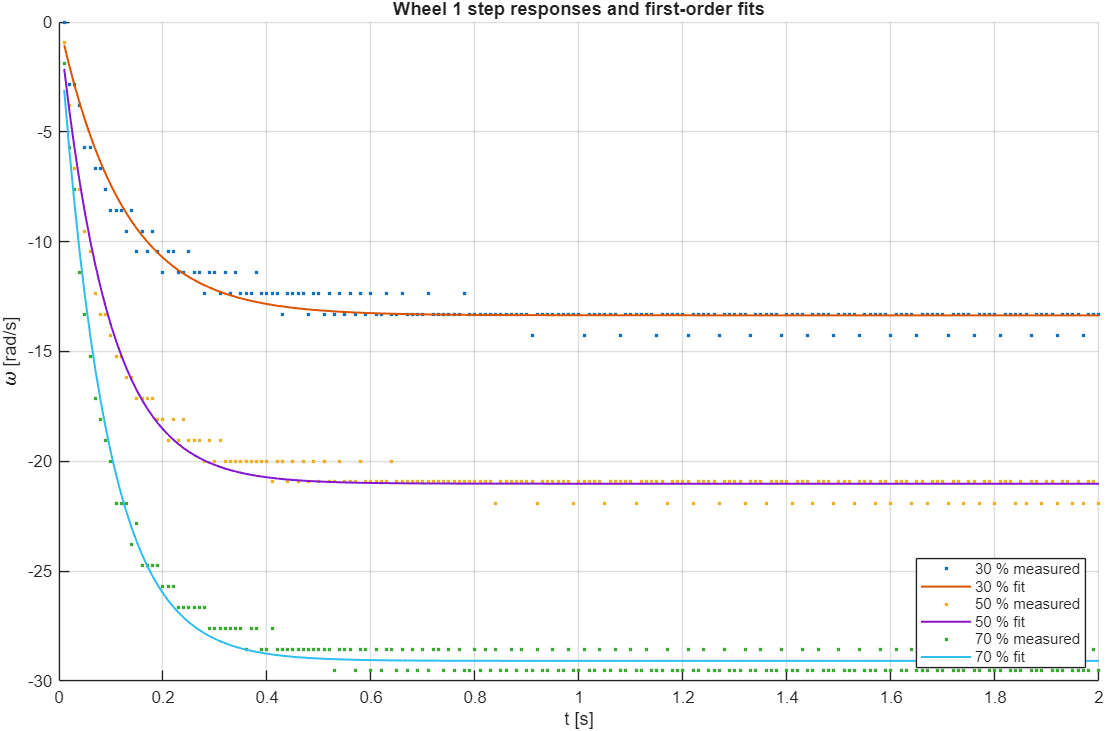
\includegraphics[width=0.8\textwidth]{e2_fit.png}
\end{center}
(The earlier fit of wheel~1 at three duties, TI1.) The rms error is about half of one count step (0.95\,rad/s in TI1), so the first-order model fits as well
as the encoder resolution allows; in TI1 and TI2 the step is 0.48\,rad/s.

\smallskip\noindent
\textbf{The four wheels} (2026-11-05, the second cart, wheels in the air, 50\,\% = 6\,V, 200 samples each, all
positive; fitted by least squares on $\tau$ with $u = 6$\,V):

\smallskip\noindent
\begin{tabular}{@{}c c c c c@{}}
\toprule
Wheel & mean $\omega$ from 1\,s (rad/s) & $K\,u$ (rad/s) & $K$ (rad/s per V) & $\tau$ (s) \\
\midrule
1 & 21.63 & 21.45 & 3.58 & 0.095 \\
2 & 20.83 & 20.60 & 3.43 & 0.106 \\
3 & 19.49 & 19.29 & 3.22 & 0.089 \\
4 & 19.07 & 18.74 & 3.12 & 0.130 \\
\bottomrule
\end{tabular}

\smallskip\noindent
The fit leaves about 0.4 to 0.6\,rad/s rms, about one count per sample (0.48\,rad/s). The fitted $K u$ is a little
below the mean from 1\,s on because the speed still creeps up slowly after the first rise, which a first-order
model cannot follow. $K$ spreads by 13\,\% between the wheels (wheel~1 the fastest, wheel~4 the slowest), which is
why A3 needs a speed controller to drive straight. The figure is what E.3 asks for, one panel per wheel:
\begin{center}
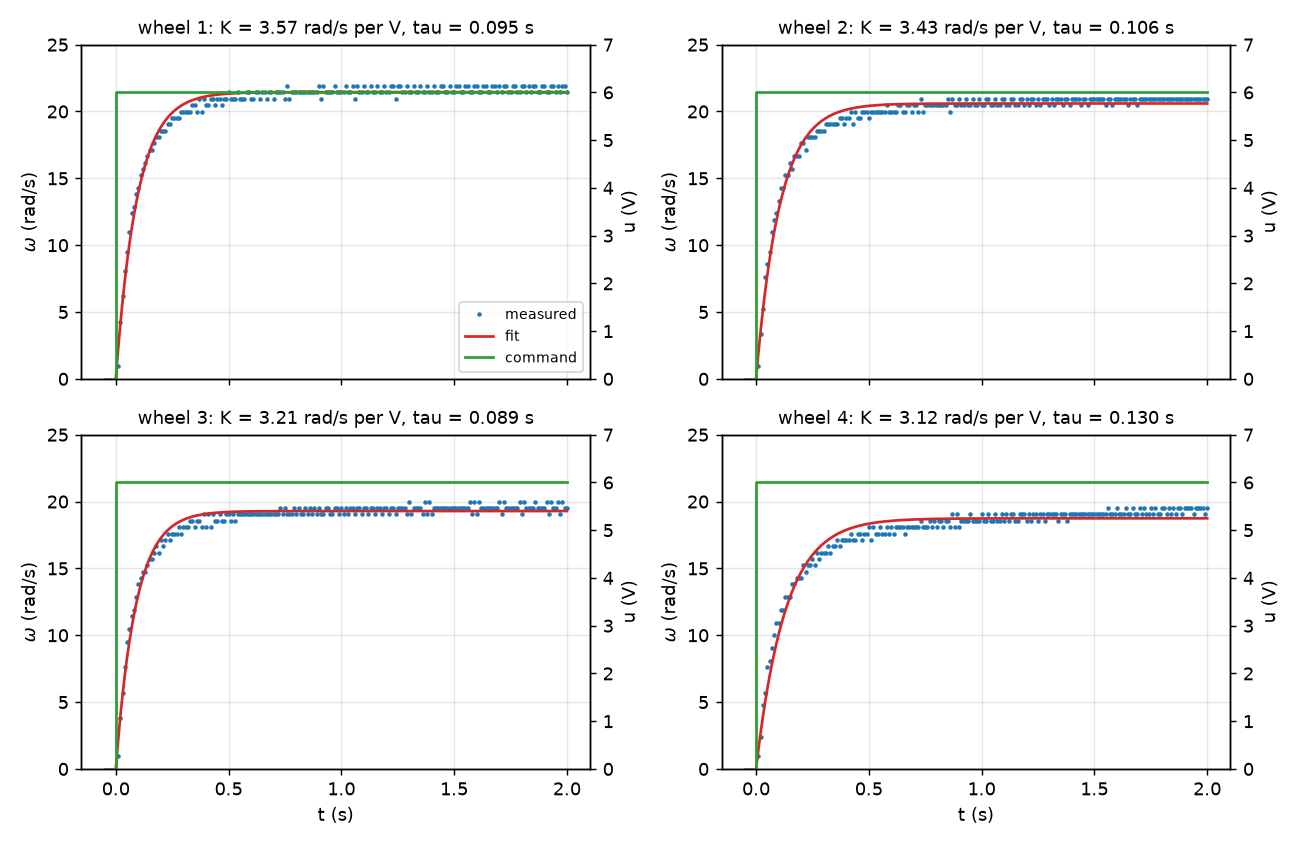
\includegraphics[width=\textwidth]{e3_wheels.png}
\end{center}

Before these runs we expected $\tau$ about 0.1\,s for all (the mechanical time constant), which holds
(0.09 to 0.13\,s), and $K$ within a few percent between the wheels, which does not: a wheel that differs much
points to friction or a worn gearbox, and students may well see a spread like ours. $K$ also changes with the battery: on
2026-10-29 the same steps of wheel~1 gave about 15\,\% less speed than on 2026-11-04.

\section{Grading notes}
\begin{itemize}
  \item The protocol (\texttt{volatile uint16\_t task}, the tags, \texttt{=== task N done ===}) is what the automatic
        test relies on (\texttt{assignments\_autotest.py}, class \texttt{Tester2}, \lv{task} written with
        \texttt{-w16}). The test presses B1 itself over SWD to end the B tasks.
  \item Part A is graded from \texttt{V\_A} (with sound), plus the code. A.1.2 must keep $M = N/2$ in the code; A.2
        must use the TIM7 callback (not the main loop). In A.2.3 the callback must stop by itself, or the task
        cannot be left. A.3 writes CCR1 only.
  \item B.1 from the report only: a linear fit of several distances, an estimate of its accuracy, and the comparison
        with the speed of sound and TIM5's clock.
  \item B: one sensor per task (B.2 the IR sensor only, B.3 the ultrasonic one only). The IR interrupt is on
        only in 222, the ultrasonic one only in 232 (and in B.1 if they use it). The polling
        tasks must not use any callback. The callbacks write only CCR1 and flags, with no I2C and no \texttt{printf}.
        LEDs and the status line only when the status changes; B1 ends every task. The shared variables are
        \texttt{volatile}. B.3 is the clearest difference (no stop with polling, one per pass with interrupts).
  \item C: no \texttt{io\_board.c} calls in Part~C. C.1 finds 7 addresses (0x03 and 0x70 as well): accept that, with
        an explanation. The register list and the reason for each value are required, and C.3 must compare with the
        times expected from the bit rate.
  \item D.1 by changing the mode at run time (no second project), counts per revolution by hand in both modes, the
        factor and why D.1.3 does not give exactly 2. D.2 in the better mode, with at least two wraps, whichever way
        the wheel counts.
  \item E: the table of the four wheels (motor, encoder, DIR level, direction, counts per revolution); recording
        inside the interrupt, printing afterwards; four \texttt{.mat} files; one figure per wheel with the speed in
        rad/s and the command in V against time in s; $K$ and $\tau$ of each wheel, compared.
\end{itemize}

\end{document}
